% Paper 2015
\documentclass[peerreviewca,11pt,a4paper]{IEEEtran}

\usepackage{ifpdf}
\usepackage{cite}

\ifCLASSINFOpdf
    \usepackage[pdftex]{graphicx}
    \graphicspath{{../pdf/}{../jpeg/}}
    \DeclareGraphicsExtensions{.pdf,.jpeg,.png}
\else
    \usepackage[dvips]{graphicx}
    \graphicspath{{../eps/}}
    \DeclareGraphicsExtensions{.eps}
\fi

\usepackage[cmex10]{amsmath}

\usepackage{array}
\usepackage{fixltx2e}

\ifCLASSOPTIONcaptionsoff
  \usepackage[nomarkers]{endfloat}
 \let\MYoriglatexcaption\caption
\renewcommand{\caption}[2][\relax]{\MYoriglatexcaption[#2]{#2}}
\fi

\usepackage{url}

\usepackage{siunitx}
\DeclareSIUnit\photon{\ensuremath{\gamma}}
\DeclareSIUnit\proton{p}
\DeclareSIUnit\neutron{n}
\DeclareSIUnit{\seivert}{Sv}

\usepackage{booktabs}

\usepackage{graphicx}
\usepackage{epstopdf}

\usepackage{caption}
\usepackage{subcaption}

\usepackage{todo}
%\renewcommand\todo[1]{\relax}
%\renewcommand\todos{\relax}

\usepackage{bpchem}
\def\U238{\BPChem{\^{238}U}}

% correct bad hyphenation here
\hyphenation{op-tical net-works semi-conduc-tor}

\begin{document}

\title{
    Detailed Geant4 simulations of the ANITA and ANITA-CUP neutron facilities
}

\author{
    \IEEEauthorblockN{
        Q. Hong\IEEEauthorrefmark{1},
        S. P. Platt\IEEEauthorrefmark{1},
        A. V. Prokofiev\IEEEauthorrefmark{2}\IEEEauthorrefmark{3} and
        E. Passoth\IEEEauthorrefmark{3}
    }
    \IEEEauthorblockA{
        \IEEEauthorrefmark{1}
        University of Central Lancashire, England
    }
    \IEEEauthorblockA{
        \IEEEauthorrefmark{2}
        Division of Applied Nuclear Physics, University of
        Uppsala, Sweden
    }
    \IEEEauthorblockA{
        \IEEEauthorrefmark{3}
        The Svedberg Laboratory, University of Uppsala, Sweden
    }
}

\maketitle

\begin{abstract}
    Simulations of the ANITA spallation neutron source at The Svedberg Laboratory (TSL) are described.
    Neutron radiation calculations show close agreement with measurements at both standard and close user positions.
    Gamma radiation characteristics are also predicted.
\end{abstract}

\IEEEpeerreviewmaketitle

\section{Introduction}

The ANITA facility~\cite{Prokofiev2009} at The Svedberg Laboratory (TSL) in Uppsala, Sweden, has been widely used for accelerated testing for neutron single-event effects (SEE).
A high-flux upgrade of the facility, ANITA-CUP, has recently been introduced and reported~\cite{Prokofiev2014}.

Platt et al. have reported preliminary Monte Carlo simulations of neutron and gamma production at the standard ANITA facility~\cite{Platt2013}.
That work was motivated by a need to understand possible sensitivity to gamma rays in detectors used for beam monitoring during SEE tests.
Simulations of a bare spallation target showed qualitative agreement with independent calculations and measurements of the fast neutron field~\cite{Prokofiev2009}.
The present work was motivated partly by a desire to investigate whether improvements to the geometry used in the simulations would lead to closer quantitative agreement with measurements, and partly by a need to extend the work to encompass the new ANITA-CUP facility~\cite{Prokofiev2014}.

Accordingly, in this paper we present a comprehensive set of analyses of neutron and gamma fields at ANITA and ANITA-CUP, with comparison to independent models and validation against measurements.
We present a subset of those results in this extended abstract.

\section{Modelling}
Simulations were conducted using Geant4 version 10.0~\cite{Agostinelli2003,Allison2006} with the binary intranuclear cascade model (see also~\cite{Platt2013}).
A detailed model of the ANITA geometry was implemented in Geant4, as illustrated in Fig.~\ref{fig:ANITAoverview}.
%; a summary only is given here.
%The spallation target is a tungsten cylinder of diameter \SI{5}{\cm} and length \SI{2.4}{\cm}~\cite{ANITAdrawing}.
%The target is cooled by water and surrounded by a stainless-steel cooling jacket.
%The target assembly with its cooling jacket appears as a small blue rectangle in Fig.~\ref{fig:ANITAoverview}.
%Lead shielding blocks in the target region are also modelled, and shown in red Fig.~\ref{fig:ANITAoverview}.
%A large electromagnet surrounding the target is modelled and shown in Fig.~\ref{fig:ANITAoverview} in grey (iron) and yellow (copper).
%An iron collimator with variable apertures is modelled  and shown downstream of the target (grey).
Simulated protons were incident axially at an energy of \SI{180}{\MeV}.
Resulting neutron and gamma fields were evaluated at several virtual detector locations.
In this paper results are presented for three of these: the Standard User Position (SUP), \SI{2.5}{\m} downstream of the target, the Close User Position (CUP), \SI{0.75}{\m} downstream of the target, and the CUP-TOF position, \SI{0.84}{m} downstream of the target.
%N.B. This is downstream of the downstream edge of the target in Qian's model.
The SUP position is downstream of a collimator with variable aperture; the CUP and CUP-TOF positions are upstream of the same collimator.
The SUP and CUP positions are of interest as they are positions used for SEE tests; the CUP-TOF position is the location of thin-film breakdown counter (TFBC) detectors used for beam monitoring and characterisation including neutron time of flight (TOF) measurements.
TFBC data are used to validate simulation results.
Except where noted otherwise, all results in this summary are for the standard collimator aperture, with \SI{10.2}{\cm} diameter.
Results for other collimator apertures will be presented in the full paper.

\begin{figure}[t]
	\centering
	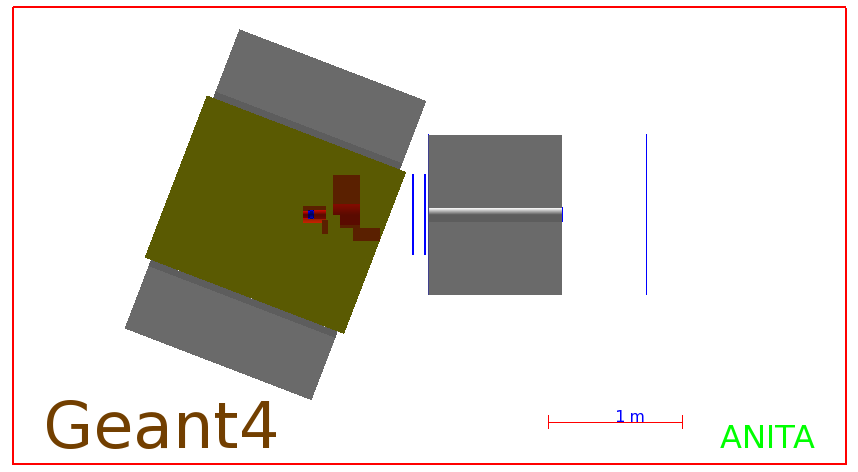
\includegraphics[width=\columnwidth]{overview.png}
	\caption{
        Simulated ANITA facility overview seen from above (yellow: bending magnet; red: shielding components; blue: neutron production target assembly; grey: collimator; blue: virtual detector system)
    }
	\label{fig:ANITAoverview}
\end{figure}

\section{Results and discussion}

\subsection{Neutrons}
Fig.~\ref{fig:SUPDensity} shows neutron distribution at the SUP, for neutrons above \SI{10}{\MeV}.
The collimator ensures that the beam is circular. Within the beam umbra the calculated neutron fluence rate above \SI{10}{\MeV} at a proton current of \SI{215}{\nA} is \SI{7.05e5}{\neutron\per\cm\squared\per\second}, compared to \SI{6.38e5}{\neutron\per\cm\squared\per\second} from earlier calculations~\cite{Platt2013} and \SI{1.0e6}{\neutron\per\cm\squared\per\second} from measurements~\cite{Prokofiev2009}.
The present calculations therefore underestimate measurements at the SUP by 30\%.

\begin{figure}[t]
    \begin{minipage}{\columnwidth}
        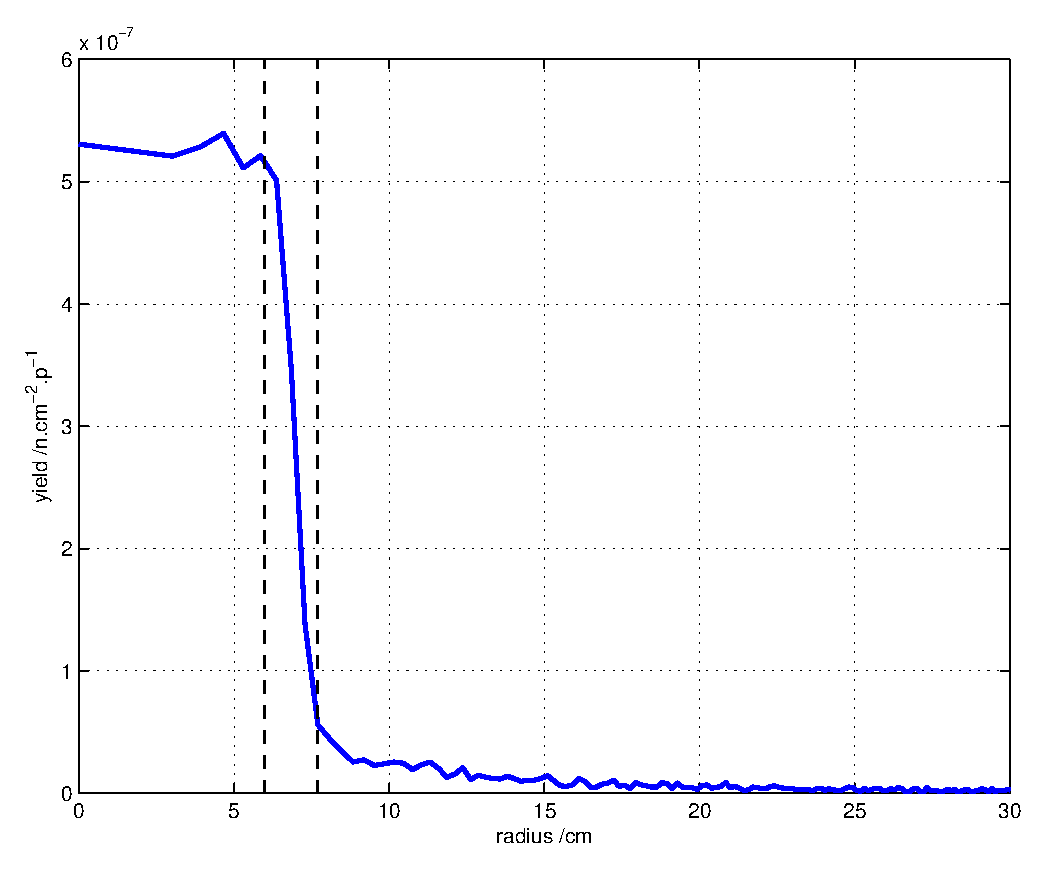
\includegraphics[width=0.9\columnwidth]{SUP10ColRadiusEffect10MeV.eps}
        \subcaption{
            Standard User Position.
            Dashed lines indicate nominal umbra and penumbra limits
        }
        \label{fig:SUPDensity}
    \end{minipage}
    \begin{minipage}{\columnwidth}
        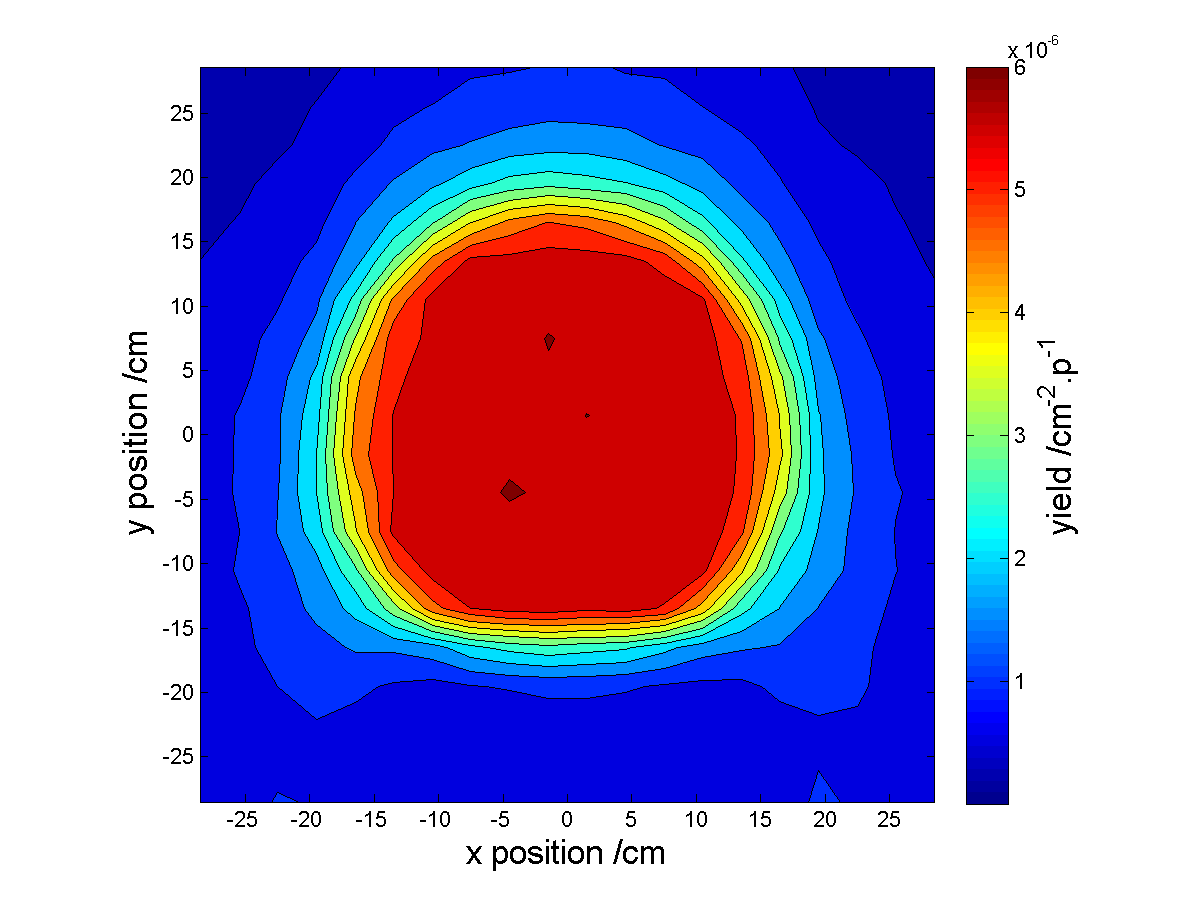
\includegraphics[width=0.9\columnwidth]{CUP10ColSpatialDistribution10MeV.png}
        \subcaption{Close User Position}
        \label{fig:CUPDensity}
    \end{minipage}
    \caption{
        Spatial distribution of neutrons above \SI{10}{\MeV} at SUP and CUP
    }
\end{figure}

\begin{figure}[!t]
    \centering
    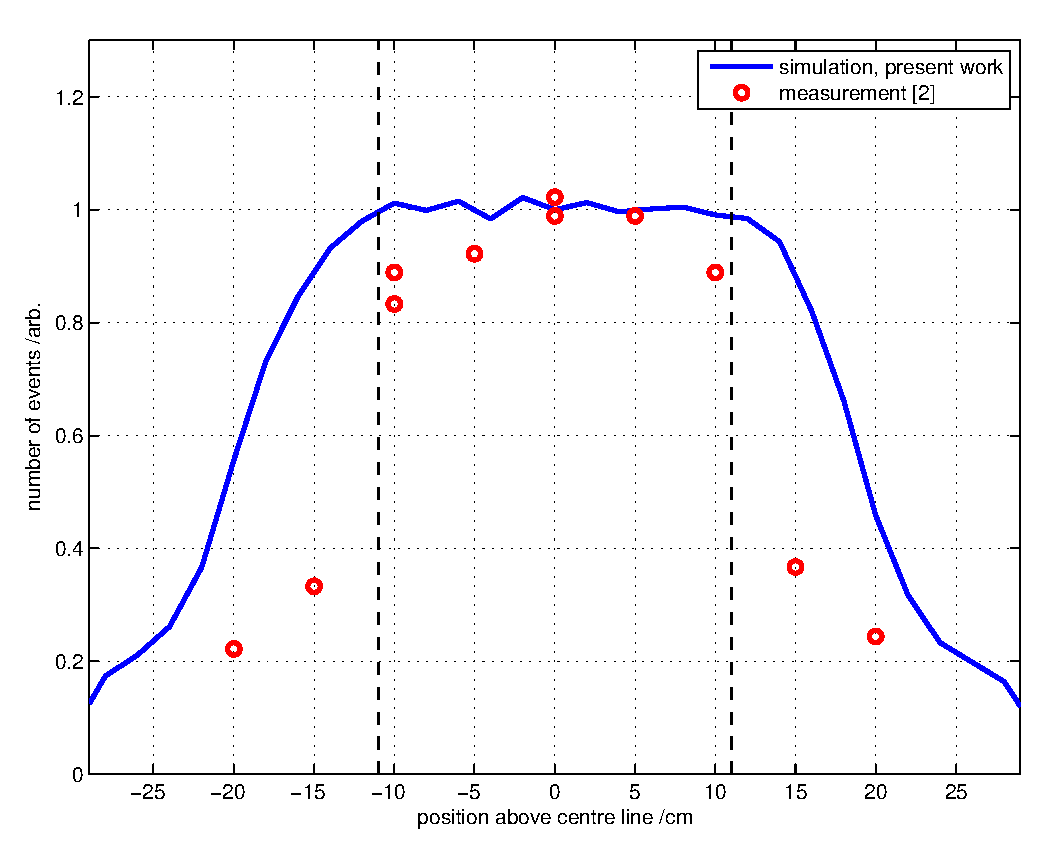
\includegraphics[width=0.9\columnwidth]{CUPTOF10beamproRADECS.eps}
    \caption{
        Vertical profile of \U238\ fission events at the CUP.
        Dashed lines indicate expected quasi-collimation by the target surroundings.
    }
    \label{fig:CUPProfile}
    \todo{Fig.~\ref{fig:CUPProfile}: add axis labels.}
\end{figure}

Fig.~\ref{fig:CUPDensity} shows the spatial distribution of neutrons above \SI{10}{\MeV} at the CUP.
As CUP is upstream of the collimator the distribution is not circularly symmetric.
In the central region the calculated neutron fluence rate above \SI{10}{\MeV} at a proton current of \SI{215}{\nA} is \SI{7.85e6}{\neutron\per\cm\squared\per\second}, compared to \SI{1.17e7}{\neutron\per\cm\squared\per\second} from measurements~\cite{Prokofiev2014}.
The present results underestimate measurements at the CUP by 33\%.

TFBCs equipped with \U238\ targets were used to measure beam profile and time of flight spectra at the CUP-TOF position.
Simulated neutron counts were folded in energy with the \U238\ fission cross-section~\cite{Carlson2009} and compared with measurements.
Fig.~\ref{fig:CUPProfile} shows the resulting vertical profiles of the neutron-induced fission rate in \U238.
The results are in general agreement although the simulation results are somewhat broader than measurements and the sharp cut-off beyond \SI{11}{\cm} is not fully reproduced by the simulation.

In Fig.~\ref{fig:TOFSpectra} we compare simulated and measured TOF spectra at the CUP-TOF position.
Neutron TOF data from the simulation were folded in energy with the \U238\ fission cross-section, convolved with a \SI{5}{\ns} rectangle function approximating the primary proton micropulse shape, and overlapped at \SI{45}{\ns}, representing the timing ambiguity due to the micropulse period.
The results show very close agreement in the position and width of the TOF peak.
The continuum beyond about \SI{30}{\ns}, corresponding to neutrons below about \SI{40}{\MeV}, is somewhat higher in the calculation than in the measurement.
This might indicate a relative overestimate of lower energy neutrons in the calculations.

Prokofiev et al.~\cite{Prokofiev2014} note that the TOF spectrum at the CUP consists of three parts, a component directly from the target, one scattered forward from target surroundings, and one scattered backwards from the front face of the collimator block.
The present simulations confirm the Prokofiev et al. semi-empirical multi-component model. Details of this confirmation will be presented in the full paper but are omitted here for brevity.

\begin{figure}[t]
    \centering
    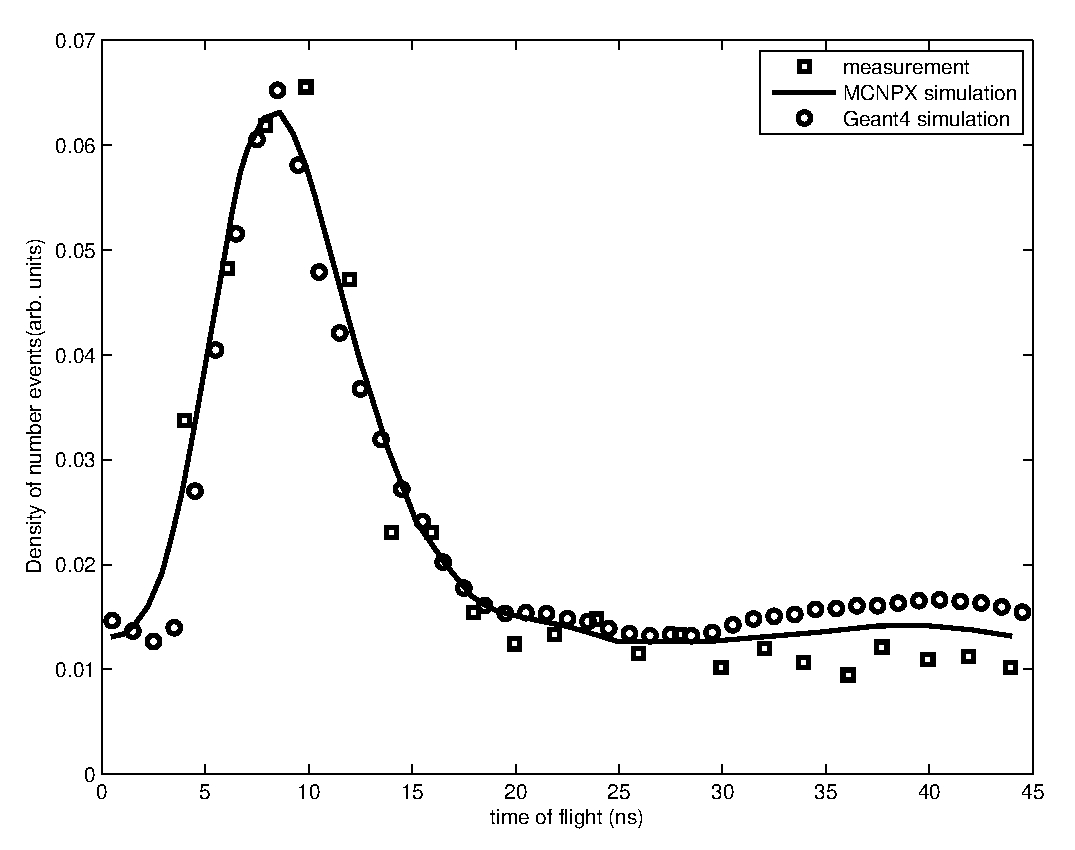
\includegraphics[width=0.9\columnwidth]{CUPTOFtofspectraRADECS.eps}
    \caption{
        Time of flight spectra for \U238 fission events at the CUP-TOF position, with \SI{3}{\cm} diameter collimator.
        }
    \label{fig:TOFSpectra}
    \todo{Fig.~\ref{fig:TOFSpectra}: correct axis labels.}
\end{figure}

\begin{figure}[t]
    \begin{minipage}{\columnwidth}
        \centering
        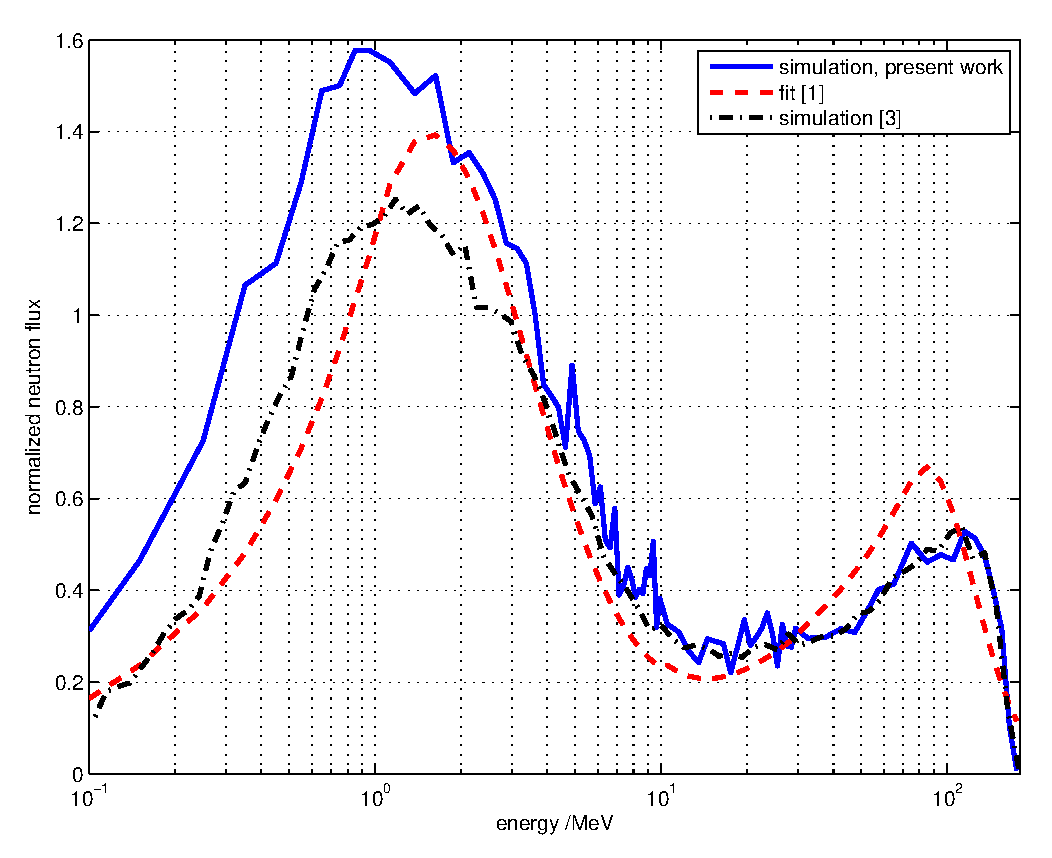
\includegraphics[width=0.9\columnwidth]{SUPNormalisedRADECS.eps}
        \subcaption{
            SUP.
            The comparison is to the fit of Prokofiev et al.~\cite{Prokofiev2009} and preliminary Geant4 modelling by Platt et al.~\cite{Platt2013}
        }
        \label{fig:LethargyplotSUP}
    \end{minipage}
    \begin{minipage}{\columnwidth}
        \centering
        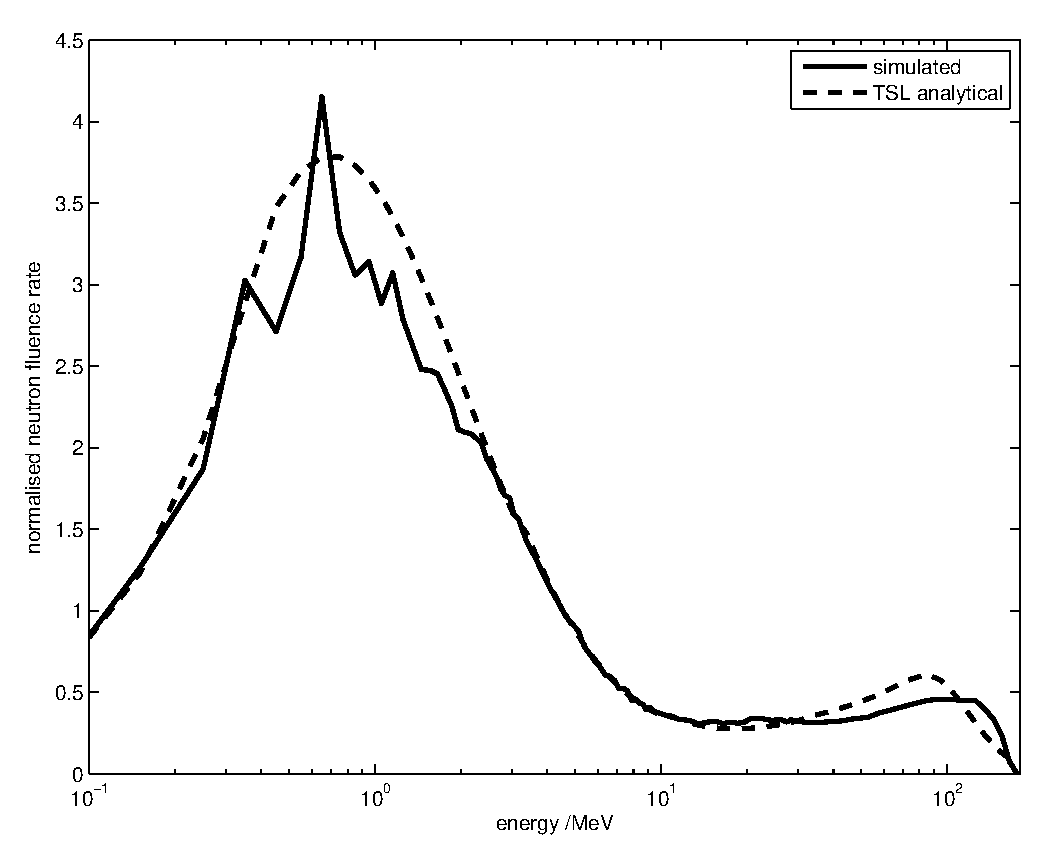
\includegraphics[width=0.9\columnwidth]{CUPcomparedProkofiev2014NormalisedRADECS.eps}
        \subcaption{
            CUP.
            The comparison is to the fit of Prokofiev et al.~\cite{Prokofiev2014}
        }
        \label{fig:LethargyplotCUP}
    \end{minipage}
	\caption{
        Calculated neutron spectra, normalised to fluence above \SI{10}{\MeV} }
	\label{fig:Lethargyplots}
\end{figure}

Fig.~\ref{fig:Lethargyplots} compares calculated spectra at SUP and CUP with analytical fits based on MCNPX simulations~\cite{Prokofiev2009,Prokofiev2014}.
The SUP data are also compared with results from Geant4 simulations of the bare target~\cite{Platt2013}.
These curves are normalised to neutron fluence above \SI{10}{\MeV} and presented as lethargy plots to emphasis the shape of the spectra rather than their integral fluence rate.
%The increased integral fluence rate at SUP from the present calculations, compared to the preliminary results of \cite{Platt2013}, is therefore not visible in Fig.~\ref{fig:LethargyplotSUP}.
The present results show an increased contribution below about \SI{1}{\MeV}, consistent with interactions in materials other than the target, absent from the preliminary simulations.
Fig.~\ref{fig:LethargyplotCUP} shows extremely close agreement between the present results and the analytical fit from~\cite{Prokofiev2014} (which cannot reproduce the structure in the evaporation peak around \SI{1}{\MeV}).

When compared to the fits the calculated spectra from the current work lead to slightly lower neutron yield and slightly higher peak energies in the higher energy peak near \SI{100}{\MeV}.
This is consistent with results for TOF spectra (see Fig.~\ref{fig:TOFSpectra} and associated discussion.)
It is not surprising that this is unaffected by the improved model geometry as this peak arises from nucleon cascades in the target.
We continue to investigate this discrepancy and will discuss it further in our final paper.

\begin{figure}[!t]
    \centering
    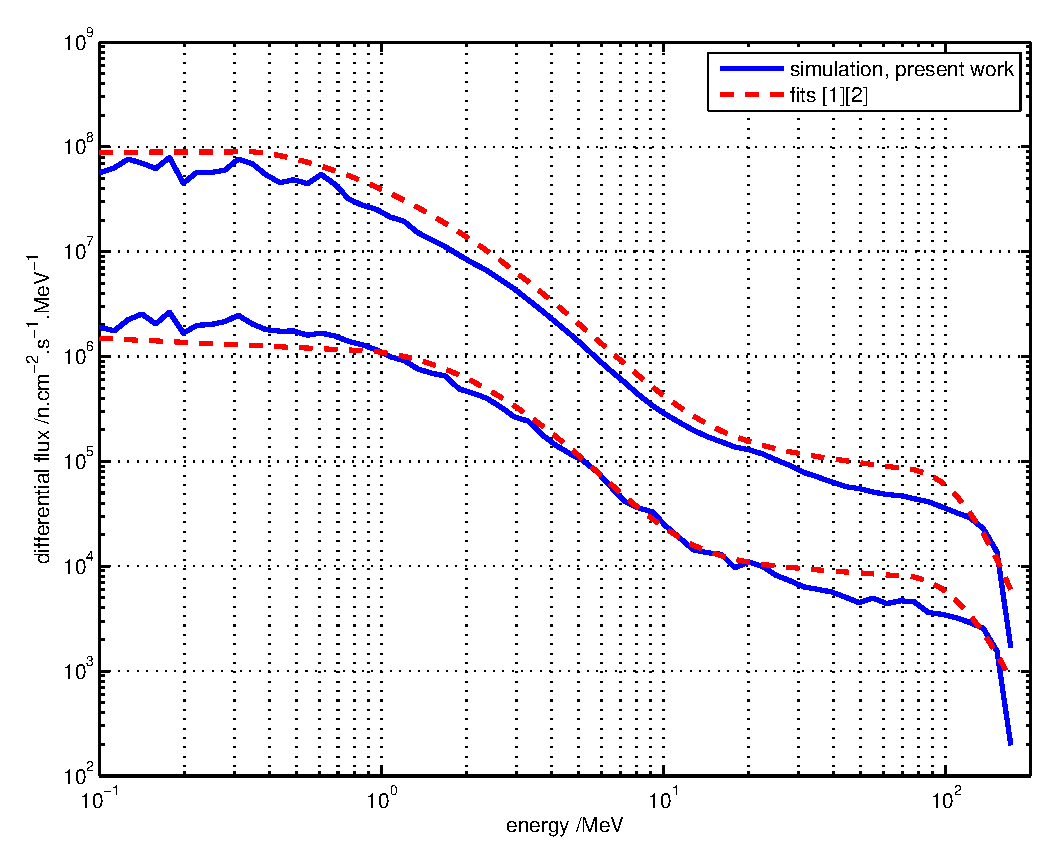
\includegraphics[width=0.9\columnwidth]{DiffYieldComparedSUPCUP10RADECS.eps}
    \caption{
        Differential neutron spectra at CUP (upper curves) and SUP (lower curves).
        Comparison is to the fits of Prokofiev et al.~\cite{Prokofiev2009,Prokofiev2014}.
    }
    \label{fig:DifferentialSpectra}
\end{figure}

Fig.~\ref{fig:DifferentialSpectra} summarises neutron spectra results by comparing differential flux as calculated in this work with the analytical fits.
The SUP calculations and fit agree very closely below \SI{20}{\MeV}; the fit exceeds the calculations somewhat above that energy.
At CUP the fit exceeds the Geant4 calculations by about 50\%, slightly more than that above \SI{20}{\MeV}.
\todo{Check differential flux comparison one the curves have been renormalised to the same current.}

\subsection{Photons}
Fig.~\ref{fig:GammaSpatialDistribution} shows the calculated spatial distribution of gamma photons at SUP and CUP, and shows a gamma radiation distribution that is qualitatively very similar to that for neutrons at both locations.
Fig.~\ref{fig:DifferentialGammaSpectra} shows the calculated differential gamma spectra within the central region of the spatial distribution.
There is a broad continuum up to an energy of about \SI{10}{\MeV}, with a peak in the fluence spectrum at about \SI{0.5}{\MeV} (where the annihilation peak is also visible).
The gamma fluence rate is an order of magnitude greater at CUP that at SUP, consistent with the closer range to the target and its immediate surroundings.
The CUP spectrum also shows a backscatter peak around \SI{0.2}{\MeV}.

\begin{figure}[t]
    \begin{minipage}{\columnwidth}
        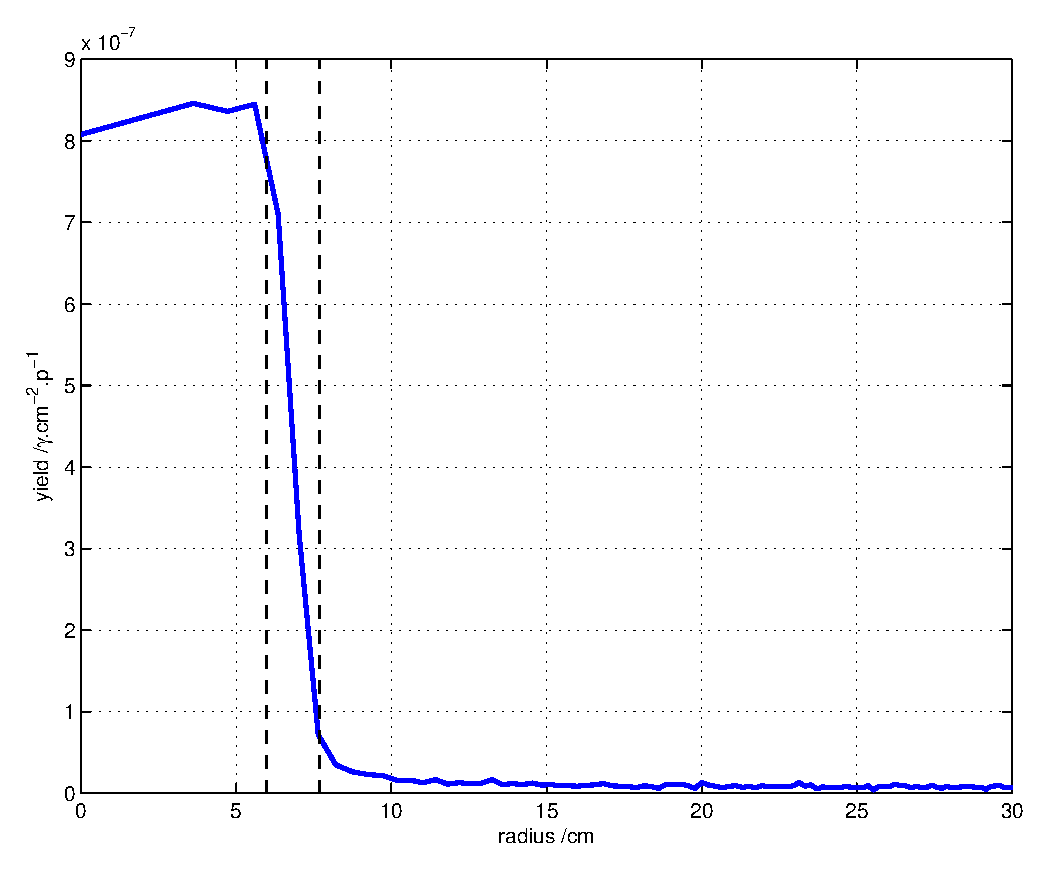
\includegraphics[width=0.9\columnwidth]{GSUPRadiusEffectaboveAllRADECS.eps}
        \subcaption{Standard User Position}
        \label{fig:GammaSpatialDistributionSUP}
    \end{minipage}
    \begin{minipage}{\columnwidth}
        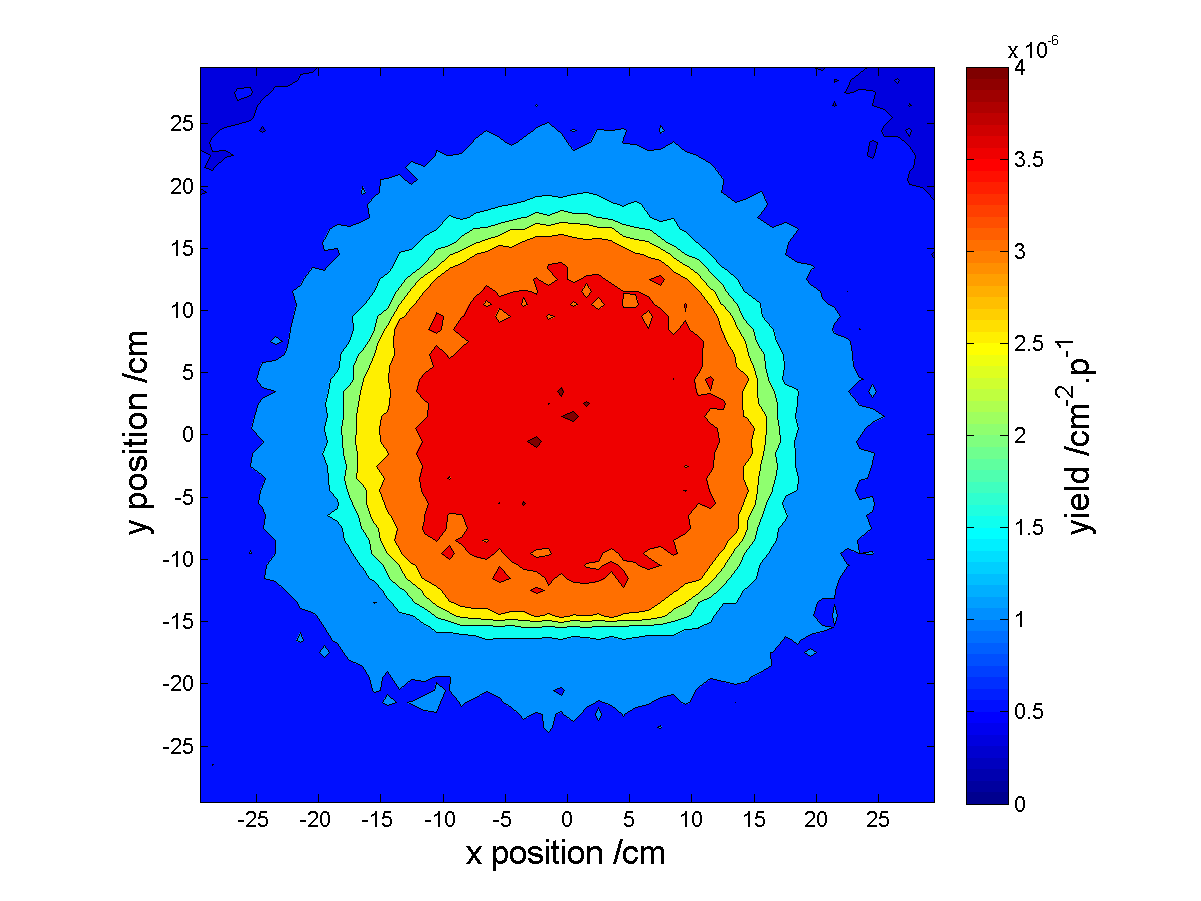
\includegraphics[width=0.9\columnwidth]{CUP10ColSpatialDistributionAllG.png}
        \subcaption{Close User Position}
        \label{fig:GammaSpatialDistributionCUP}
    \end{minipage}
    \caption{
        Calculated gamma spatial distribution
    }
    \label{fig:GammaSpatialDistribution}
\end{figure}

\begin{figure}[t]
    \centering
    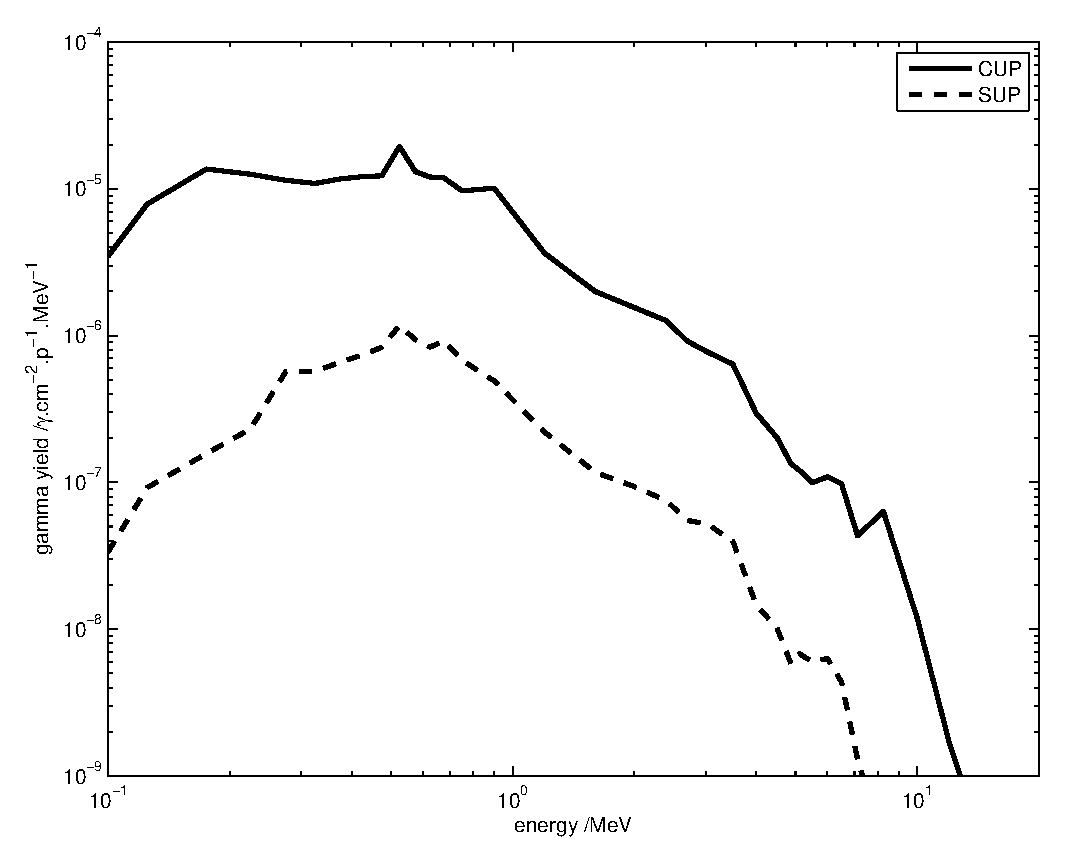
\includegraphics[width=0.9\columnwidth]{gDYieldcomparedRADECS.eps}
    \caption{
        Calculated gamma spectra at CUP (upper curve) and SUP (lower curve) }
    \label{fig:DifferentialGammaSpectra}
\end{figure}

\begin{figure}[t]
    \centering
    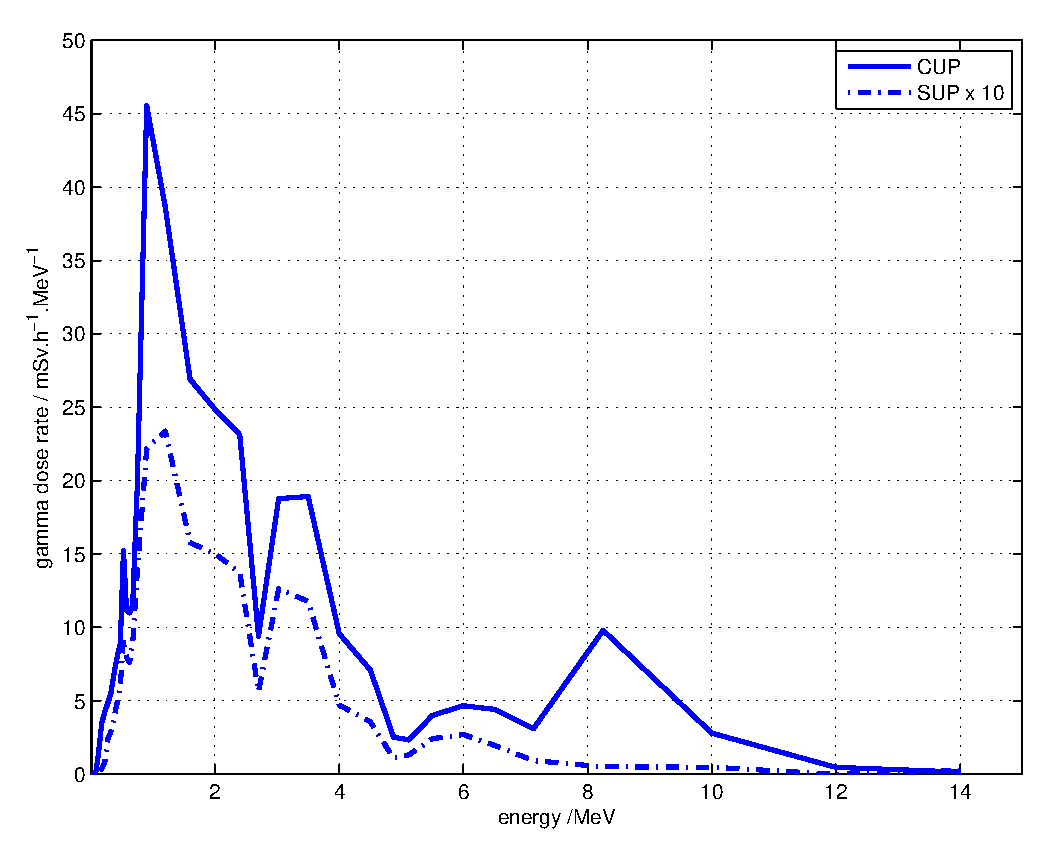
\includegraphics[width=0.9\columnwidth]{DoseVSenergycomparedRADECS.eps}
    \caption{
        Calculated gamma dose spectra }
    \label{fig:GammaDoseEnergy}
    \todo{Fig.~\ref{fig:GammaDoseEnergy}: correct y axis units.}
\end{figure}

Fig.~\ref{fig:GammaDoseEnergy} shows the calculated gamma dose spectrum, obtained by folding the gamma spectra (Fig~\ref{fig:GammaDoseEnergy}) with dose conversion data from \cite{Kwon1980}.
The results show structure with peaks around \SI{1.5}{\MeV}, \SI{3}{\MeV}, \SI{6}{\MeV} and \SI{9}{\MeV}.
Note that these are not coincidence peaks, as the simulation counts individual photons.
\todo{Discuss photon counting with Qian.}
The calculated dose rate at \SI{200}{\nA} primary proton current is \SI{21}{\milli\seivert\per\hour} at SUP and \SI{370}{\milli\seivert\per\hour} at CUP.
The calculated value at SUP is slightly more than and therefore consistent with that predicted from a bare spallation target (\SI{17}{\milli\seivert\per\hour}) and is also consistent with an estimated upper limit of \SI{40}{\milli\seivert\per\hour} reported in~\cite{Prokofiev2009}.
The calculated value at CUP is consistent with that calculated at SUP (a ratio of 17:1 is somewhat greater than $1/R^2$, as would be expected), but rather more than the estimated upper limit (\SI{170}{\milli\seivert\per\hour}) given in \cite{Prokofiev2014}.
We continue to evaluate our gamma calculations and will discuss them at greater length in the final paper.

\section{Conclusion}
We have used Geant4 for detailed Monte Carlo simulations of the ANITA and ANITA-CUP neutron SEE test facilities at The Svedberg Laboratory.
Neutron fluence rate, energy spectrum, time profile and spatial distribution show good agreement with measurements and independent simulations (using MCNPX).
Gamma radiation characteristics have also been predicted and preliminary evaluations indicate that they are consistent with a limited set of measurement data.
For reasons of space only a small subset of results are presented here.
Evaluation of our results is still in progress; additional data and evaluation will be presented in our final paper.

\begin{thebibliography}{9}
\bibitem{Prokofiev2009}
A.V. Prokofiev et al.,
\newblock ``Characterization of the ANITA neutron source for accelerated SEE testing at The Svedberg Laboratory'',
\newblock {\em 2009 IEEE Radiat. Effects Data Workshop Record}, pp.~166-173

\bibitem{Prokofiev2014}
A.V. Prokofiev et al.,
\newblock ``CUP--A new high-flux irradiation position at the ANITA neutron facility at TSL'',		\newblock {\em IEEE Trans. Nucl. Sci.} vol.~61 no.~4, pp.~1929-1936, 2014

\bibitem{Platt2013}
S. P. Platt et al.,
\newblock ``Neutron and gamma fields at neutron spallation sources for single-event-effects testing'',
\newblock {\em Proc. 14th European Conf. Radiat. Effects Compon. Syst.}, 2013

\bibitem{Agostinelli2003}
S. Agostinelli et al.,
\newblock``Geant4--a simulation toolkit'',
\newblock {\em Nucl. Inst. Meth. Phys. Res. A} vol.~506, pp.~250--303, 2003

\bibitem{Allison2006}
J. Allison et al.,
\newblock ``Geant4 developments and applications'',
\newblock {\em IEEE Trans. Nucl. Sci.} vol.~53 no.~1, pp.~270--278, 2006

\bibitem{Carlson2009}
A. D. Carlson et al.,
\newblock ``International evaluation of neutron cross section standards'',
\newblock{\em Nucl. Data Sheets} vol.~110 no.~12, pp.~3215-3324, 2009

\bibitem{Kwon1980}
S.-G. Kwon et al.,
\newblock ``Calculation of neutron and gamma-ray flux-to-dose-rate conversion factors'',
\newblock{\em J. Kor. Nucl. Soc.} vol.~12 no.~3, pp.~171-179, 1980

\end{thebibliography}

\cleardoublepage

\todos

\end{document} 